\documentclass[12pt,a4paper]{article}
\usepackage[romanian]{babel}
\usepackage{fontspec}
\setmainfont{Latin Modern Roman}
\usepackage{geometry}
\geometry{margin=2.5cm}
\usepackage{graphicx}
\usepackage{enumitem}
\usepackage{framed}

\title{AMSS 2026 — Examen restanță \\ \large (model orientativ)}
\author{Traian-Florin Șerbănuță}
\date{2026}

\begin{document}
\maketitle

\begin{framed}
\noindent\textbf{Acesta este un MODEL}, care arată \emph{structura}
subiectului de la restanță. Subiectul real va folosi \textbf{un alt
scenariu} și \textbf{alt set de artefacte}. Artefactele de mai jos sunt
pe domeniul de la curs (bike-sharing) și conțin defecte
\textbf{ilustrative}, pentru exersat — nu sunt subiectul de examen.
\end{framed}

\bigskip

\textbf{Durată:} 90 de minute. \textbf{Format:} test scris, fără AI.

\noindent Testul verifică nivelul minim de competență
(F1 + F3 + F4 din specificația cursului): citirea critică a
artefactelor UML generate de AI, articularea raționamentului de design,
și apărarea trasabilității. Artefactele furnizate sunt generate de AI și
\emph{conțin defecte} — sarcina ta este să le găsești, să explici cum ai
dirija AI, și să aperi trasabilitatea.

\section*{Specificația sistemului (exemplu)}

O aplicație de bike-sharing oferă închirieri de biciclete. Cerințele
identificate sunt:

\begin{description}[leftmargin=3.2em,style=nextline]
  \item[R1] O \textbf{închiriere} (Rental) este pentru exact o bicicletă
        și un utilizator.
  \item[R2] Utilizatorul ia o bicicletă dintr-o \textbf{stație}; stația
        \textbf{deține} biciclete care îi supraviețuiesc oricărei
        închirieri.
  \item[R3] O bicicletă trece prin stările: disponibilă, rezervată, în
        uz; o bicicletă cu defect intră în \textbf{mentenanță} și revine
        disponibilă după reparație.
\end{description}

\section*{Artefacte furnizate (generate de AI)}

\paragraph{Diagrama de clase.}

\begin{center}
  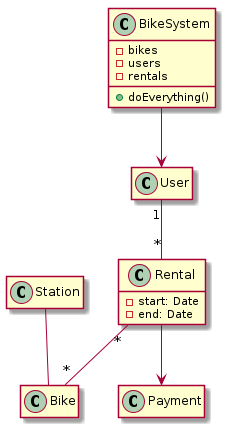
\includegraphics[width=\linewidth,height=8cm,keepaspectratio]{sample-class}
\end{center}

\paragraph{Diagrama de stare a bicicletei (Bike).}

\begin{center}
  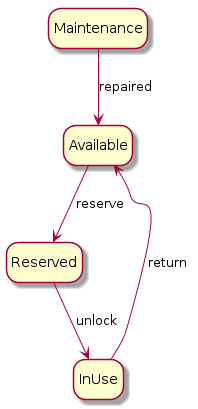
\includegraphics[width=\linewidth,height=8cm,keepaspectratio]{sample-state}
\end{center}

\newpage

\section*{Partea I — Critică (F1)}

Identificați defectele din cele două artefacte de mai sus.
Găsiți \textbf{cel puțin cinci} defecte. Pentru fiecare, specificați:

\begin{enumerate}
    \item Locul defectului (ce artefact, ce element).
    \item Categoria (multiplicitate greșită, clasă-zeu, infrastructură
          inventată, agregare lipsă, stare orfană / fără ieșire, guard
          lipsă, fabricație, vagitate etc.).
    \item Severitatea (critică / majoră / minoră).
    \item Corecția propusă.
\end{enumerate}

\vspace{5.5cm}

\section*{Partea II — Raționament (F3)}

\textit{Dată cerința R3:} o bicicletă trece prin stările disponibilă,
rezervată, în uz, iar una cu defect intră în mentenanță și revine
disponibilă după reparație.

Cum ați dirija un AI pentru a produce \textbf{diagrama de stare a
bicicletei} care respectă R3? Ce ați respinge din output-ul tipic al
AI-ului și de ce?

\vspace{5.5cm}

\section*{Partea III — Trasabilitate (F4)}

\textit{Dată cerința R1:} o închiriere este pentru exact o bicicletă.

Identificați inconsistența dintre R1 și diagrama de clase (care arată
relația \texttt{Rental "*" -- "*" Bike}). Parcurgeți lanțul de
trasabilitate — de la cerință la element de model — care expune
problema, și spuneți cum ar trebui corectat.

\vspace{5.5cm}

\end{document}
